% Generated by scripts/build-paper.py — edit paper/src/survey.src.md
\section{Evidence synthesis}\label{sec:evidence-synthesis}

\subsection{The evidence base}

The thirteen core studies appeared over four days, beginning four days after the launch (Figure 1). Relationships overlap: 10 studies evaluate or use hosted Jev, 5 build or evaluate independent Jev-like models, and 6 embed typed decisions in a larger system (Table 3). Of the 11 studies that query hosted Jev, 8 state the version they called (\texttt{jev-1.13.0} or \texttt{jev-1.13}; one uses \texttt{typesafe/jev1.13} through OpenRouter \citep{arxiv2609_24574}) and 3 state none. Every core study is an arXiv v1 preprint.

\begin{figure}[tbp]
\centering
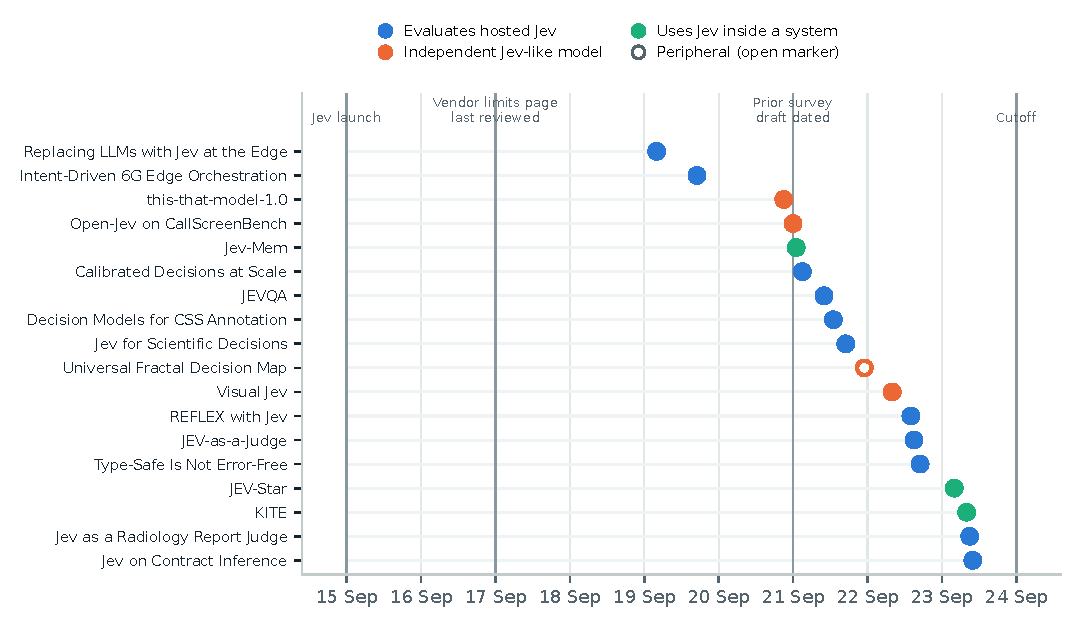
\includegraphics[width=\linewidth]{figures/timeline.pdf}
\caption{Submission dates of the core and peripheral studies (arXiv v1) against context events, by primary relationship to Jev.}\label{fig:timeline}
\end{figure}

\begin{table}[tbp]
\centering\footnotesize
\caption{Core and peripheral studies (* peripheral; † same study family). Headline values are author-reported.}\label{tab:core}
\begin{tabularx}{\linewidth}{p{0.2\linewidth}p{0.055\linewidth}p{0.085\linewidth}p{0.11\linewidth}Xp{0.075\linewidth}}
\toprule
\textbf{Study} & \textbf{v1 (2026)} & \textbf{Test level} & \textbf{Version} & \textbf{Headline (as reported)} & \textbf{Ref.} \\
\midrule
Replacing LLMs with Jev at the Edge † & 09-19 & Hybrid & jev-1.13 & Median client decision latency −15.9\% to −26.5\% & \citep{arxiv2609_22753} \\
Intent-Driven 6G Edge Orchestration † & 09-19 & Hybrid & Jev 1.13 & Median decision latency −22.4\% vs DeepSeek, −61.9\% vs Gemini & \citep{arxiv2609_23136} \\
this-that-model-1.0 & 09-20 & Model test & 1.0; not reported & 30.9 ms per decision on one laptop GPU; 32 decisions/s & \citep{arxiv2609_23886} \\
Open-Jev on CallScreenBench & 09-21 & Model test & paper v1 (three seeds) & JevLite ensemble AUROC .974, ECE .052; no false alarms & \citep{arxiv2609_23959} \\
Jev-Mem & 09-21 & System test & not reported & LoCoMo judge 0.777 (+11.0\%); build 158 s; 0.93 s/query & \citep{arxiv2609_23986} \\
Calibrated Decisions at Scale & 09-21 & System test & jev-1.13.0 & 499,500 narratives screened for \$25.23; 195,857 fully coded & \citep{arxiv2609_24052} \\
JEVQA & 09-21 & Model test & jev-1.13 & PLCC vs VMAF: 0.737 (metadata) → 0.824 (+bitstream, pixel) & \citep{arxiv2609_24395} \\
Decision Models for CSS Annotation & 09-21 & Model test & typesafe/jev1.13 & Behind best LLM on 14/15 tasks (−11.6 F1) at 44× lower cost & \citep{arxiv2609_24574} \\
Jev for Scientific Decisions & 09-21 & System test & Jev 1.13 & Full semantic correctness; median 0.335 s, p95 0.442 s & \citep{arxiv2609_24965} \\
Universal Fractal Decision Map * & 09-21 & Model test & not reported & Self-reported 92.6\% macro-accuracy, 7.08 ms on CPU, “\#1” on JevBench & \citep{arxiv2609_25498} \\
Visual Jev & 09-22 & Model test & paper v1 & Macro accuracy 0.706 → 0.761 after post-training (seen families) & \citep{arxiv2609_25845} \\
REFLEX with Jev & 09-22 & System test & jev-1.13.0 & 95\% success with 1.12 strong calls/task vs 88\% and 4.10 (−72.7\%) & \citep{arxiv2609_26532} \\
JEV-as-a-Judge & 09-22 & Model test & jev-1.13.0 & RewardBench 92.2\% vs 93.5\%; HaluEval 87.5\% vs 86.7\% (GPT-6) & \citep{arxiv2609_26550} \\
Type-Safe Is Not Error-Free & 09-22 & Model test & not reported & Hosted Jev AUROC .8146 → .5806 after name–rubric swap; 0\% type errors & \citep{arxiv2609_26758} \\
\bottomrule
\end{tabularx}
\end{table}

\subsection{F1 · A type-valid answer can still be the wrong answer}

Typed interfaces remove parse and schema failures by construction, and nothing more. In the most direct test, the authors held question, state, rubric wording and the set of option names fixed and changed only which name was bound to which rubric \citep{arxiv2609_26758}. For hosted Jev, rebinding the rubrics behind \emph{no/yes} flipped 32.50\% of answers, against 2.08\% and 1.67\% under neutral names. It lowered balanced accuracy from .7127 to .5163 and AUROC from .8146 to .5806 on 1,200 items. The swap produced 24× the model's test–retest floor, while the type-error rate stayed at 0\% in every condition. The larger reversal in the abstract, AUROC .9376 → .2315, belongs to an open marker-readout head, not to Jev. That head is also where neutral renaming of multi-way options changed 52.42\% of answers. Random character-string names returned flip rates to the neutral regime without costing accuracy, which suggests that polarity, not naming itself, drives the effect. Community audits add closed-set and primitive effects. Removing an abstain option drove accuracy on unanswerable items from 0.950 to 0.000 at 0.79 confidence, and a Noul and a two-option Choice over the same question differed by 0.125 on average \citep{gh_jujumilk3_jev_calibration_audit}. In a synthetic-panel study, the choice of primitive reversed a comparison with GPT-4.1 \citep{gh_jjd_lab_jev_synthetic_survey}. In agents, reliability depends on the size of the action set and on near-valid alternatives near authorisation boundaries \citep{arxiv2609_26532}. In scientific workflows, wrong selections changed derived counts while the final label stayed correct \citep{arxiv2609_24965}. The vendor's own list of weaknesses — literal reading, arithmetic, dates, indirection, large irrelevant state and adversarial text — points the same way \citep{typesafe2026jaggedness}.

Two qualifications matter. Order is a different intervention from binding: one community audit saw no argmax flips in 400 order permutations on hosted Jev \citep{gh_jujumilk3_jev_calibration_audit}, whereas frozen open readouts are order-sensitive until calibrated \citep{gh_nokia_applied_research_anyjev}. And the mitigations the authors propose (neutral identifiers, randomised names in training) have not been evaluated. Related work outside the Jev literature reaches the same conclusion from other directions: schema descriptions act as prompts \citep{arxiv2608_08254}, forced forms invite invented answers \citep{arxiv2607_20492}, and tool-using agents fail by binding the right action to the wrong entity \citep{arxiv2606_30531}.

\subsection{F2 · A native probability makes calibration measurable, not guaranteed}

Every call returns a distribution, so reliability can be audited on each run. Measured reliability varies. Across 15 computational-social-science tasks, Jev's median ECE was 0.157 (95\% CI 0.108–0.233). That beat the verbalised confidence of 16 of 19 LLMs but not three frontier Claude models (best 0.066) \citep{arxiv2609_24574}. The same study shows how a global average hides a local failure: on empathy in peer-support dialogues the model was confident while near chance, a task ECE of 0.538. On crash narratives, probabilities ranked well but overstated prevalence. Recalibration fitted on half of 2,416 blinded human judgments cut calibration error by about 3.3×, and calibration varied by model rather than by paradigm \citep{arxiv2609_24052}. Community audits disagree across datasets. One pre-registered audit found ECE 0.0204 on CLINC150 and 0.0936 on Banking77 \citep{gh_jourdanlabs_assay_001}. Another found that a temperature of about 3.4 was needed on a task whose rule is not recoverable from the text \citep{gh_scienthoon_jev_ood_calibration}. A third found that a Spanish state cost 3.0–6.4 accuracy points and doubled ECE on the hardest tasks \citep{gh_marcosmartinez_jev_acento}. Open models show the same pattern: JevLite reaches calibration error .052 with a temperature-scaled two-label readout, but on synthetic calls and with a recipe chosen under test-set exposure \citep{arxiv2609_23959}.

The qualifications are specific. Native confidence is essentially the maximum probability \citep{arxiv2609_26550}, and the vendor presents calibration as a group property \citep{typesafe2026systemone}. The probabilities are quantised to two decimals \citep{arxiv2609_24052}. The background literature explains the rest: calibration degrades under shift \citep{arxiv1906_02530}; the ranking of confidence signals changes out of domain \citep{arxiv2608_19558}; answer-preserving attacks can move confidence readouts \citep{arxiv2608_06571}; and conformal certificates can fail under a change in how scores are produced \citep{arxiv2609_04445}. Calibration is therefore a property to verify per workload and per construct, with recalibration on held-out target labels. It is not a certificate.

\subsection{F3 · A bounded first pass with confidence-gated escalation}

Across judging, annotation and agent control, the typed model is usually the cheapest and fastest component, and rarely the most accurate. As a judge, Jev stayed within three points of the strongest comparator (GPT-6 Astra) on ordinary preference and evidence-grounded factuality: 92.2\% vs 93.5\% on RewardBench and 87.5\% vs 86.7\% on HaluEval. A frozen two-order cascade kept 99\% of the comparator's accuracy at 57\% of its fee \citep{arxiv2609_26550}. In agent control, a Jev-gated agent reached 95\% success with 1.12 strong-model calls per task against 88\% and 4.10 calls for a strong-only agent \citep{arxiv2609_26532}. In annotation, Jev trailed the per-task best LLM on 14 of 15 tasks (median −11.6 macro-F1) at a median 44× lower cost. Routing its low-confidence items to an LLM matched or exceeded the LLM alone at a quarter to half of the cost \citep{arxiv2609_24574}. On crash narratives the typed model reached F1 0.908 against human labels, and one frontier model was 0.059 higher \citep{arxiv2609_24052}.

Every one of these gains is conditional. Thresholds chosen on a selection set did not transfer for every fallback, and simulated cascade fees say nothing about real cascade latency \citep{arxiv2609_26550}. On BFCL and τ-style episodes, where ordinary routing is already accurate, a cheap generative cascade remained competitive \citep{arxiv2609_26532}. Trained feature models still beat zero-shot JEVQA on video quality \citep{arxiv2609_24395}. On multi-step arithmetic, an open typed model trails strong reasoning models \citep{arxiv2609_23886}. The prior art is also clear. Cascades and routers have long traded cost against quality \citep{arxiv2305_05176,arxiv2406_18665,arxiv2601_07206}. In one recent comparison a cheap trained ensemble beat every LLM configuration outright, and a hybrid escalated only its least-confident predictions to an LLM \citep{arxiv2609_17977}. The lesson for RQ4 is to include cheap trained and generative cascades as baselines, and to fix thresholds on data separate from the test set.

\subsection{F4 · Speed and cost claims decompose into different mechanisms and scopes}

Speed figures in this literature measure different things (Table 4). Single-request latencies include 0.335 s median for scientific Choices \citep{arxiv2609_24965}, 64.5 ms for JevLite on a consumer GPU \citep{arxiv2609_23959} and 30.9 ms for this-that-model on a laptop GPU \citep{arxiv2609_23886}. Visual Jev's 5.7 ms is amortized over 32 questions sharing one image: the batch takes about 182 ms \citep{arxiv2609_25845}. End-to-end figures include network, queueing and retries \citep{arxiv2609_26550,arxiv2609_22753}. Electricity-only marginal cost excludes hardware and operations and cannot be compared with an API bill \citep{arxiv2609_23886}. Several mechanisms produce speed-ups: avoiding autoregressive decoding (JevLite's 4.9× on the same backbone), prefix sharing and batching (Visual Jev's 8.9× and 3.4×), and caching. Caching alone largely removed the latency advantage of Jev over a structured-output LLM in an edge service \citep{arxiv2609_22753}. Faster decisions did not raise end-to-end success: in a real image service reached over simulated radio access, Jev completed 459 of 1,080 requests correctly and on time, against 463 for DeepSeek \citep{arxiv2609_23136}. Serving systems explain part of the effect independently of the model \citep{arxiv2312_07104}. For RQ3 the answer is that no single speed or cost number describes a typed decision model; each figure is valid only within its scope.

\begin{table}[tbp]
\centering\footnotesize
\caption{Speed and cost figures grouped by measurement scope. Figures in different groups are not comparable.}\label{tab:scopes}
\begin{tabularx}{\linewidth}{p{0.2\linewidth}Xp{0.1\linewidth}}
\toprule
\textbf{Scope} & \textbf{Reported figure} & \textbf{Ref.} \\
\midrule
Single request & Full semantic correctness; median 0.335 s, p95 0.442 s & \citep{arxiv2609_24965} \\
Single request & 64.5 ms/decision; 4.9× faster than same backbone generating & \citep{arxiv2609_23959} \\
Single request & 30.9 ms per decision on one laptop GPU; 32 decisions/s & \citep{arxiv2609_23886} \\
Single request & Median decision latency −22.4\% vs DeepSeek, −61.9\% vs Gemini & \citep{arxiv2609_23136} \\
Single request & Median client decision latency −15.9\% to −26.5\% & \citep{arxiv2609_22753} \\
Single request & Self-reported 92.6\% macro-accuracy, 7.08 ms on CPU, “\#1” on JevBench & \citep{arxiv2609_25498} \\
Amortized per question & 8.9× vs serial, 3.4× vs no-reuse batch; 5.7 ms/question amortized & \citep{arxiv2609_25845} \\
End to end & 0.36\% of the comparator’s fee; ≈\$0.04 per 1,000 judgments at 0.15 s & \citep{arxiv2609_26550} \\
End to end & 95\% success with 1.12 strong calls/task vs 88\% and 4.10 (−72.7\%) & \citep{arxiv2609_26532} \\
End to end & Behind best LLM on 14/15 tasks (−11.6 F1) at 44× lower cost & \citep{arxiv2609_24574} \\
End to end & Low-confidence routing matches the LLM at ¼–½ of its cost & \citep{arxiv2609_24574} \\
End to end & 499,500 narratives screened for \$25.23; 195,857 fully coded & \citep{arxiv2609_24052} \\
End to end & LoCoMo judge 0.777 (+11.0\%); build 158 s; 0.93 s/query & \citep{arxiv2609_23986} \\
End to end & Correct \& on time: Jev 459, DeepSeek 463, Qwen 435 of 1,080 & \citep{arxiv2609_23136} \\
End to end & No cache: e2e −11.1–25.3\%; fees per correct completion −69–71\% & \citep{arxiv2609_22753} \\
End to end & Repeated-request caching largely removes the latency gap & \citep{arxiv2609_22753} \\
Simulated & Frozen two-order cascade: 99\% of GPT-6 accuracy at 57\% of its fee & \citep{arxiv2609_26550} \\
Simulated & Simulated completion +3.50 / +8.35 points & \citep{arxiv2609_23136} \\
Author estimate & \$0.000217 electricity per suite pass vs \$10.636 for a hosted model & \citep{arxiv2609_23886} \\
Vendor claim & No type errors by construction; plotted 0\% is analytical & \citep{typesafe2026launch} \\
Vendor claim & \$0.042 / M input tokens; 70–500 ms end to end (vendor) & \citep{typesafe2026launch} \\
Vendor claim & 193.6× faster, 444.6× cheaper on vendor workflow evals & \citep{typesafe2026launch} \\
\bottomrule
\end{tabularx}
\end{table}

\subsection{F5 · Interface compatibility is not mechanism equivalence}

§6 established that the request and response shape can be served by encoders, frozen or fine-tuned decoders, diffusion reads and prompted generators. The evidence adds three points. First, readout matters more than a “typed head” label. JevLite's gain over generation comes from reading two label logits on the same backbone, and a ModernBERT encoder was not significantly worse \citep{arxiv2609_23959}; Visual Jev's typed head gave no consistent gain \citep{arxiv2609_25845}. Second, comparisons between open and commercial models are fragile. this-that-model's 0.941 vs Jev's 0.765 on a third party's 68 questions rests on 12 items, and its 0.844 vs 0.803 on 2,250 questions uses question shapes the open model was trained on \citep{arxiv2609_23886}. Third, several projects state explicitly that they do not reproduce the commercial model \citep{gh_theoleecj_semif,gh_githubnext_localjev,gh_jaredpalmer_kev}. Typed primitives with confidence-gated execution also appear independently in data systems \citep{arxiv2608_20630}.

\subsection{F6 · System-level gains need module-level attribution}

Systems improve for many reasons at once. Jev-Mem reports a LoCoMo judge score of 0.777 (+11.0\% relative), memory construction in 158 s and 0.93 s per query. Each figure is measured against a different baseline, and the quality metric is itself an LLM judge \citep{arxiv2609_23986}. JEVQA's quality depends mainly on feature engineering: metadata-only PLCC 0.737 rose to 0.824 with bitstream and pixel features, while a pixel-only variant failed \citep{arxiv2609_24395}. The choice of reference matters as much as the model. Administrative crash codes understated narrative fidelity by a median 0.26 kappa \citep{arxiv2609_24052}, and correct final labels concealed wrong intermediate quantities in scientific workflows \citep{arxiv2609_24965}. Attribution needs ablations, matched baselines and references that measure what the workflow reuses.

\subsection{F7 · The evidence is young, clustered and unreplicated}

Thirteen core preprints appeared within four days, each as a single version (Figure 2). Two form one study family \citep{arxiv2609_23136,arxiv2609_22753}. The hosted model is non-deterministic: the test–retest floor was up to 1.33\% answer flips \citep{arxiv2609_26758}, and 50 identical requests produced 15 distinct answers in one audit \citep{gh_jujumilk3_jev_calibration_audit}. Several comparisons rest on small or test-informed samples. The recipe selection in one study had test-set exposure \citep{arxiv2609_23959}, and the 68-question comparison above rests on 12 items. The peripheral study reports “0.0\% injection bypass” with a 95\% interval up to 30.8\% \citep{arxiv2609_25498}. The vendor's workflow evaluations use model outputs as references \citep{typesafe2026launch}. None of the core results has been independently reproduced, and several claimed releases of code and raw predictions could not be located (§9).

\begin{figure}[tbp]
\centering
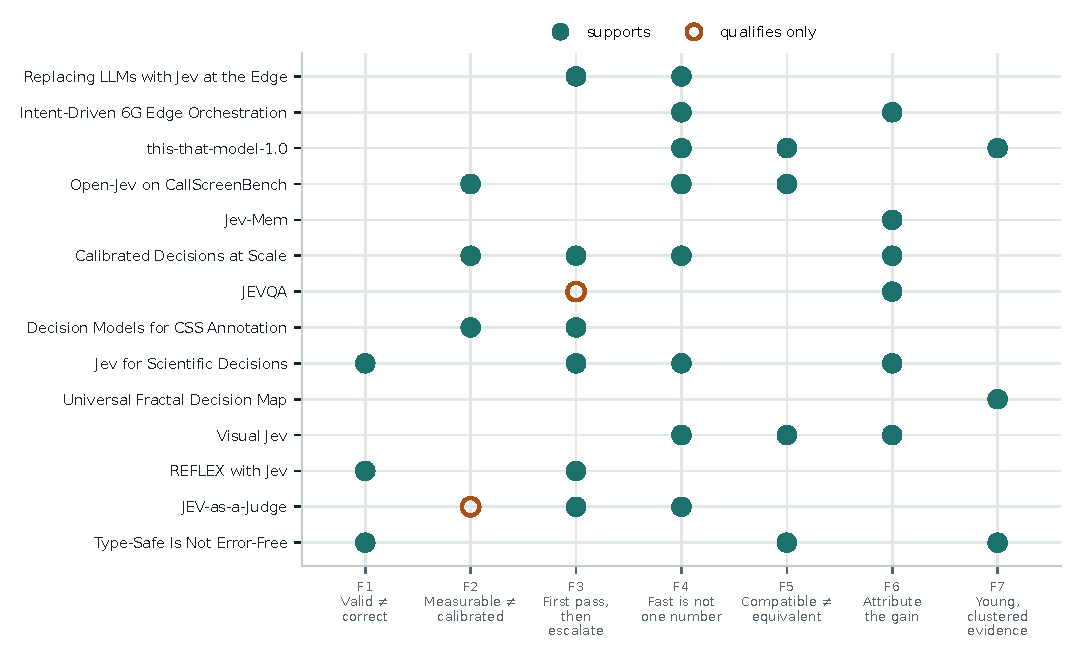
\includegraphics[width=\linewidth]{figures/matrix.pdf}
\caption{Which study bears on which finding, derived from the evidence records (filled: supports; half: qualifies).}\label{fig:matrix}
\end{figure}
